
\renewcommand{\EntradaBibtex}{Reporte2017_Tetris3D}

\begin{frame}{\citetitle{\EntradaBibtex} \footnotemark[1] (1)}
\begin{block}{Motivación} 
Este proyecto esta inspirado en un tetris 3D para PC \url{http://users.csc.calpoly.edu/~zwood/teaching/csc471/finalproj24/gzipkin/}
\begin{itemize}
\item Varias piezas caen sobre una rejilla y el objetivo es borar las lineas.
\item Las piezas se mueven en un entorno tridimensional (ejes X, Y y Z)
\item Las fronteras de la red estan definidas mediante una malla alámbrica
\item La cámara tambien se puede mover en base a eventos de toque sobre la pantalla del dispositivo
\end{itemize}
\end{block} 
\footnotetext[1]{\fullcite{\EntradaBibtex}}
\end{frame}


\begin{frame}{Aplicación Tetris 3D (2)}
%\begin{block}{Pantallas Principales} 
\begin{center}
	\begin{tabular}{cccc}
		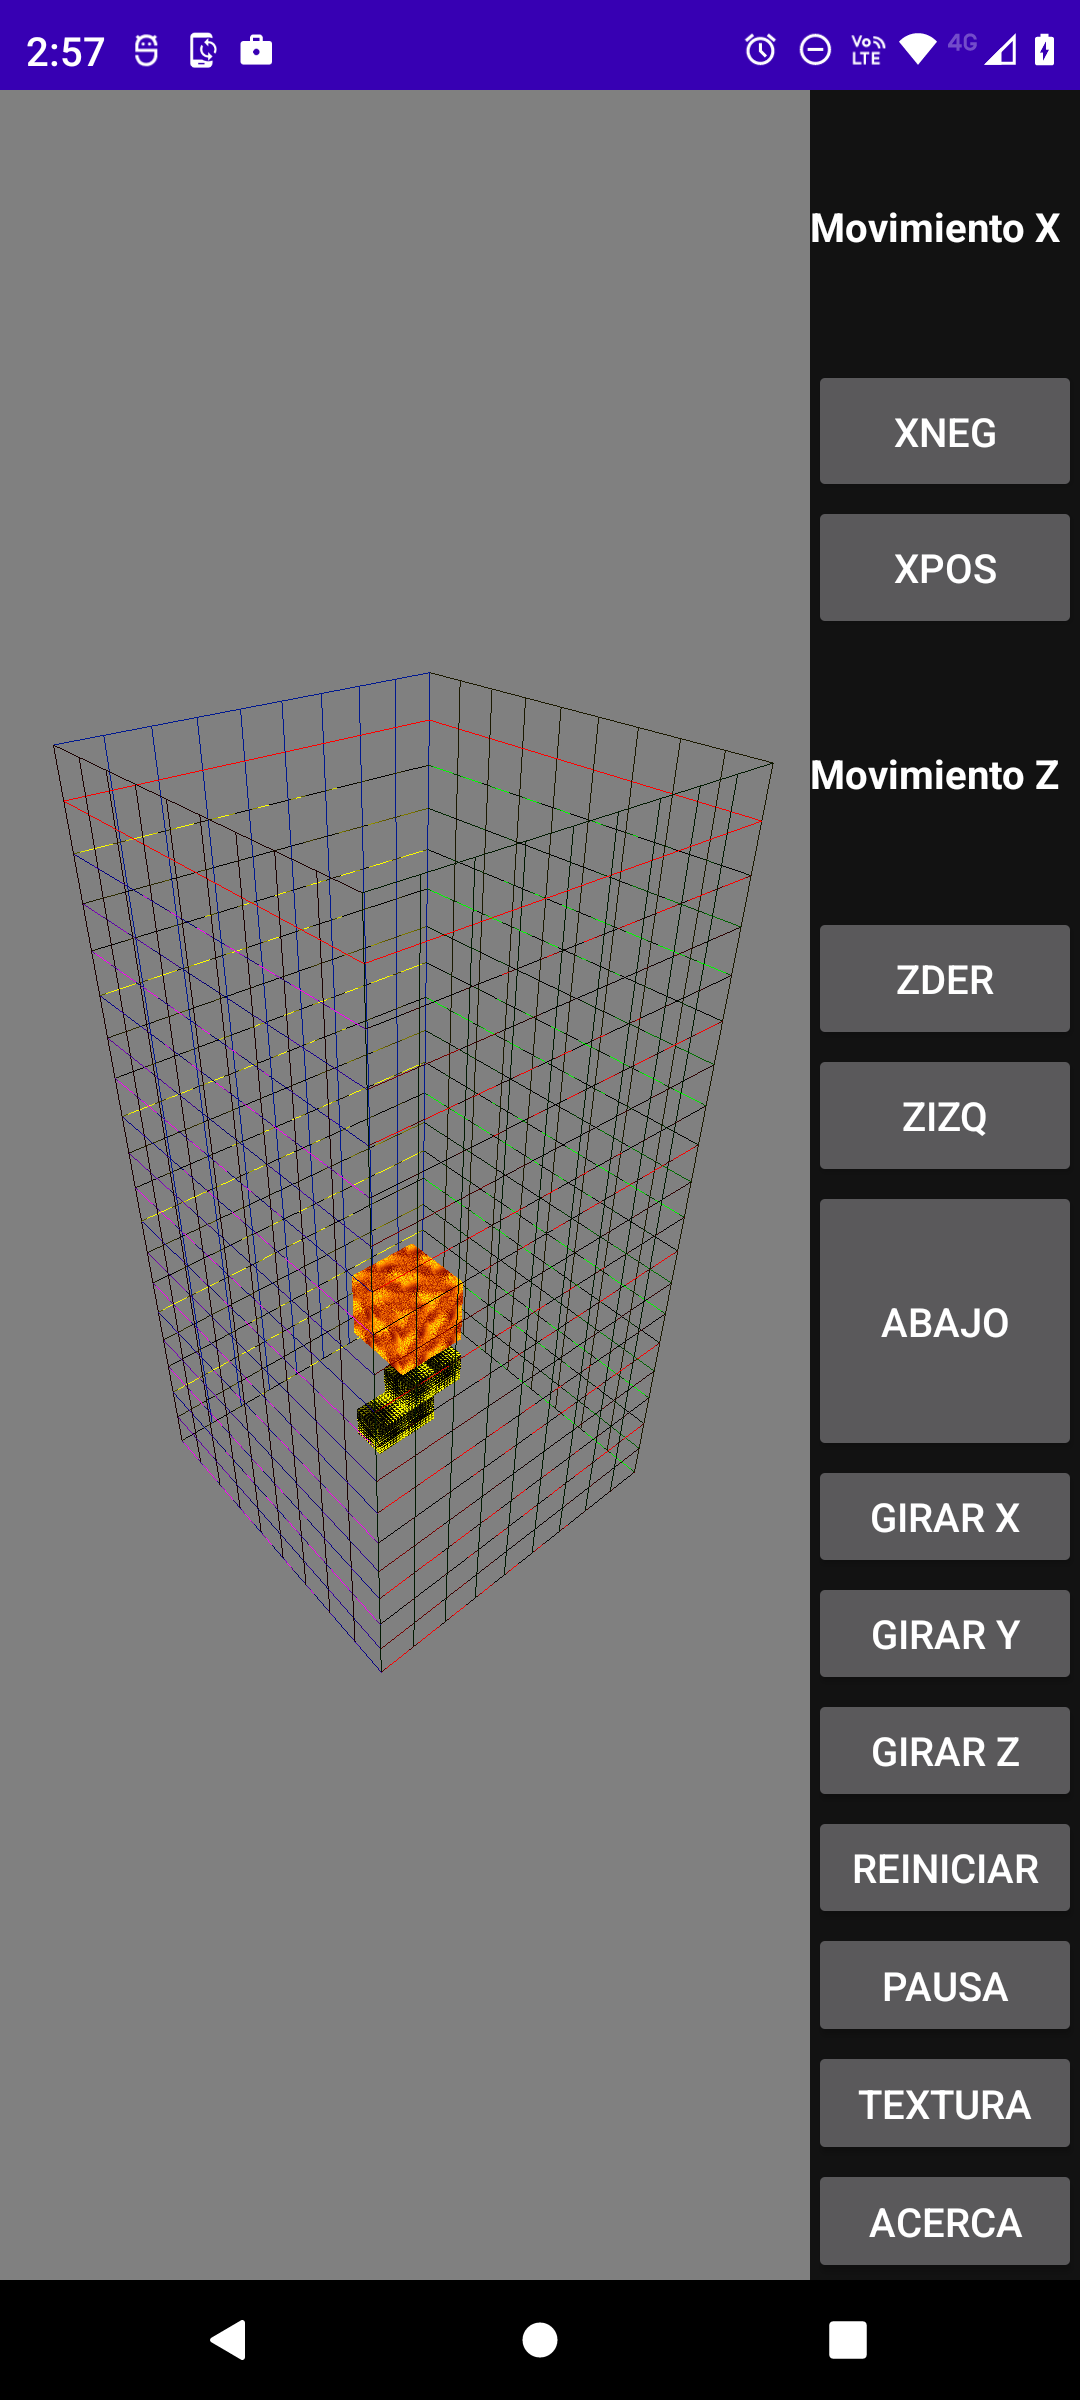
\includegraphics[width=0.20\linewidth]{2017_Tetris3D/figs/Tetris0.png} &
		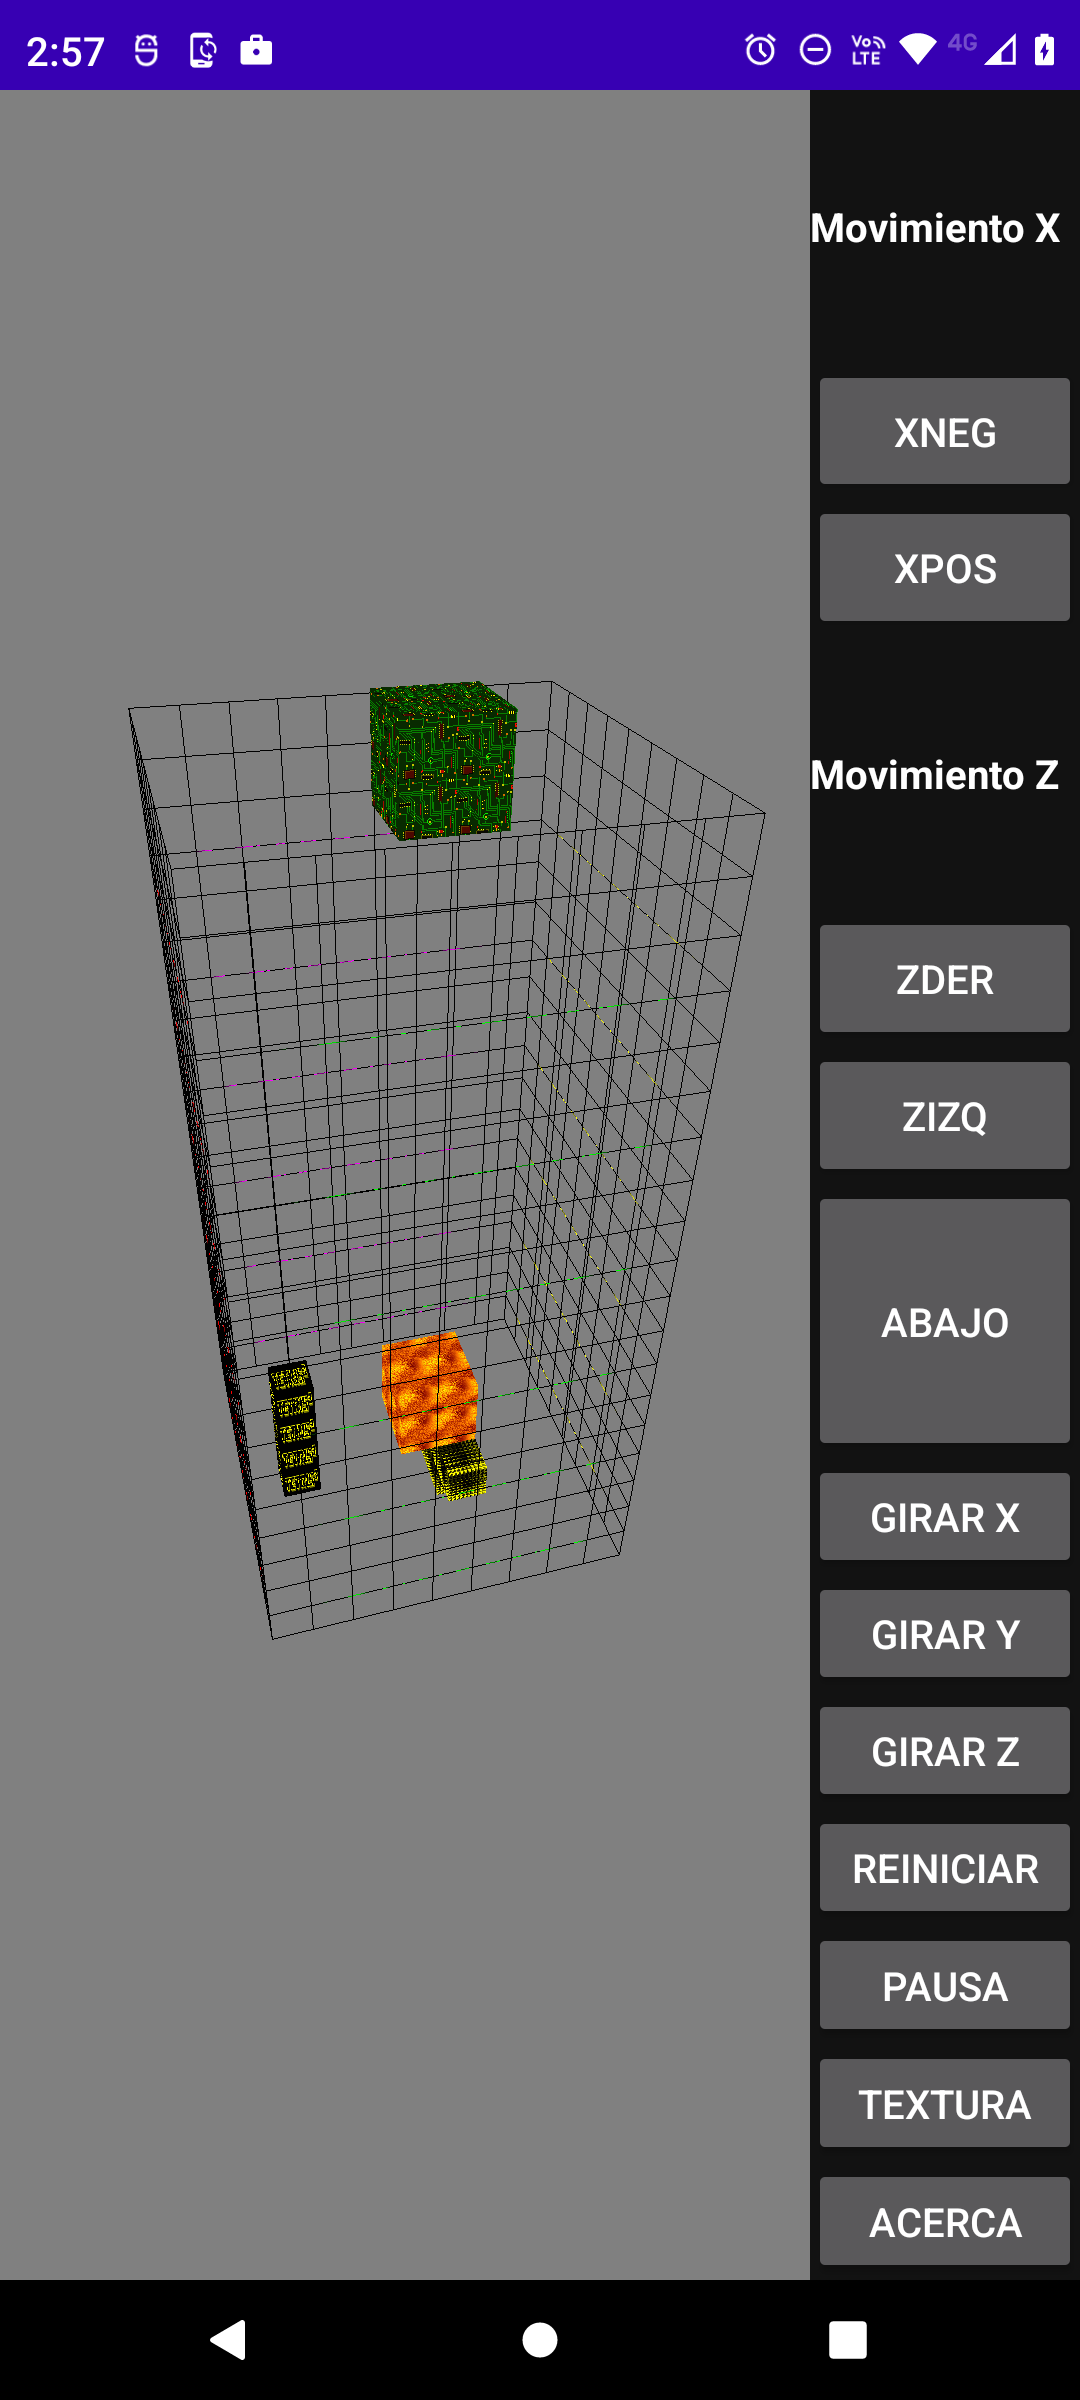
\includegraphics[width=0.20\linewidth]{2017_Tetris3D/figs/Tetris1.png} & 		 		
		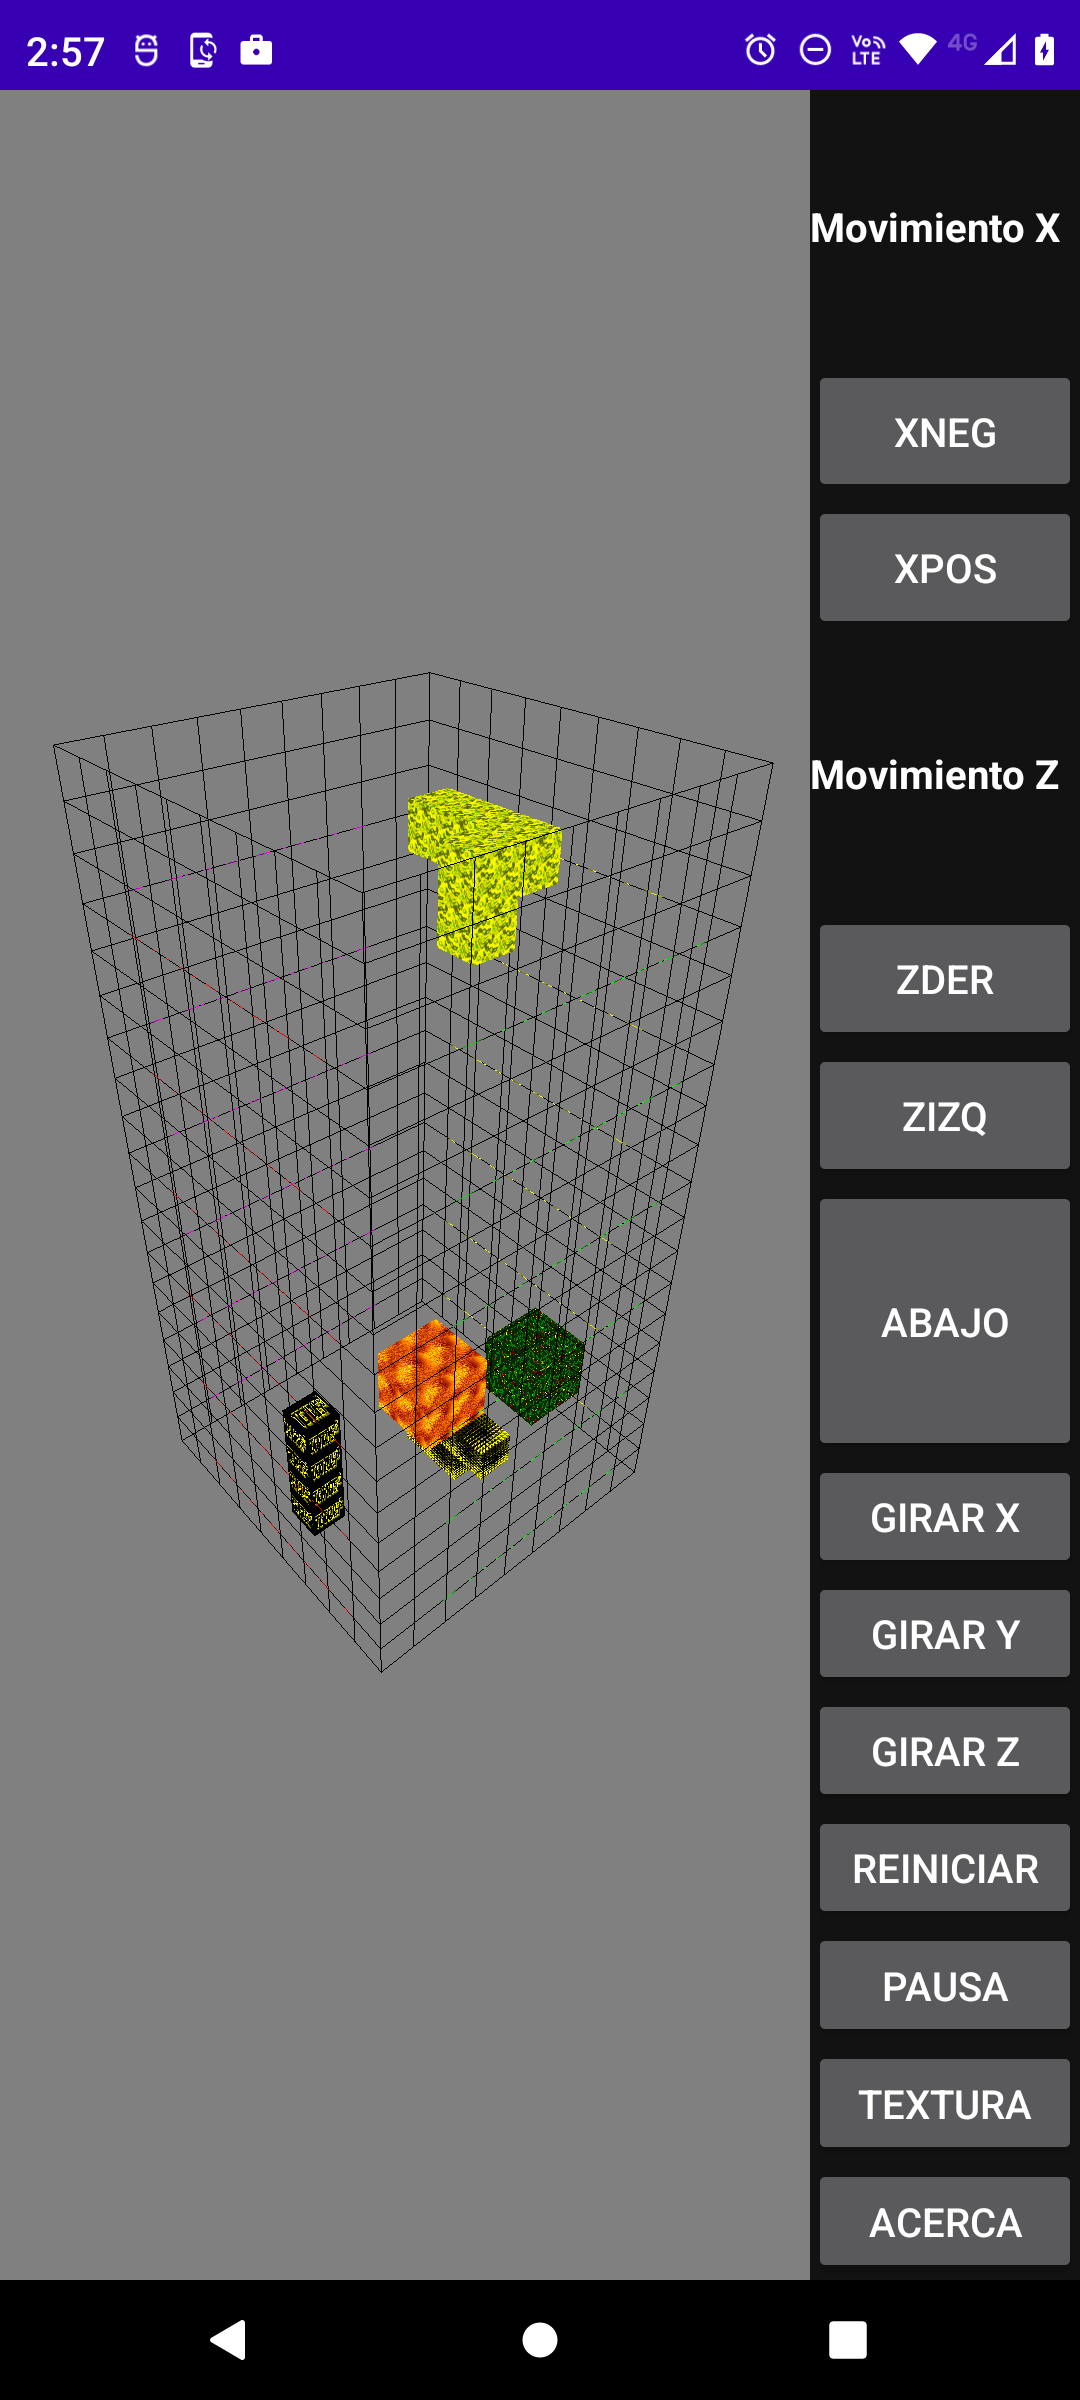
\includegraphics[width=0.20\linewidth]{2017_Tetris3D/figs/Tetris2.png} & 		
		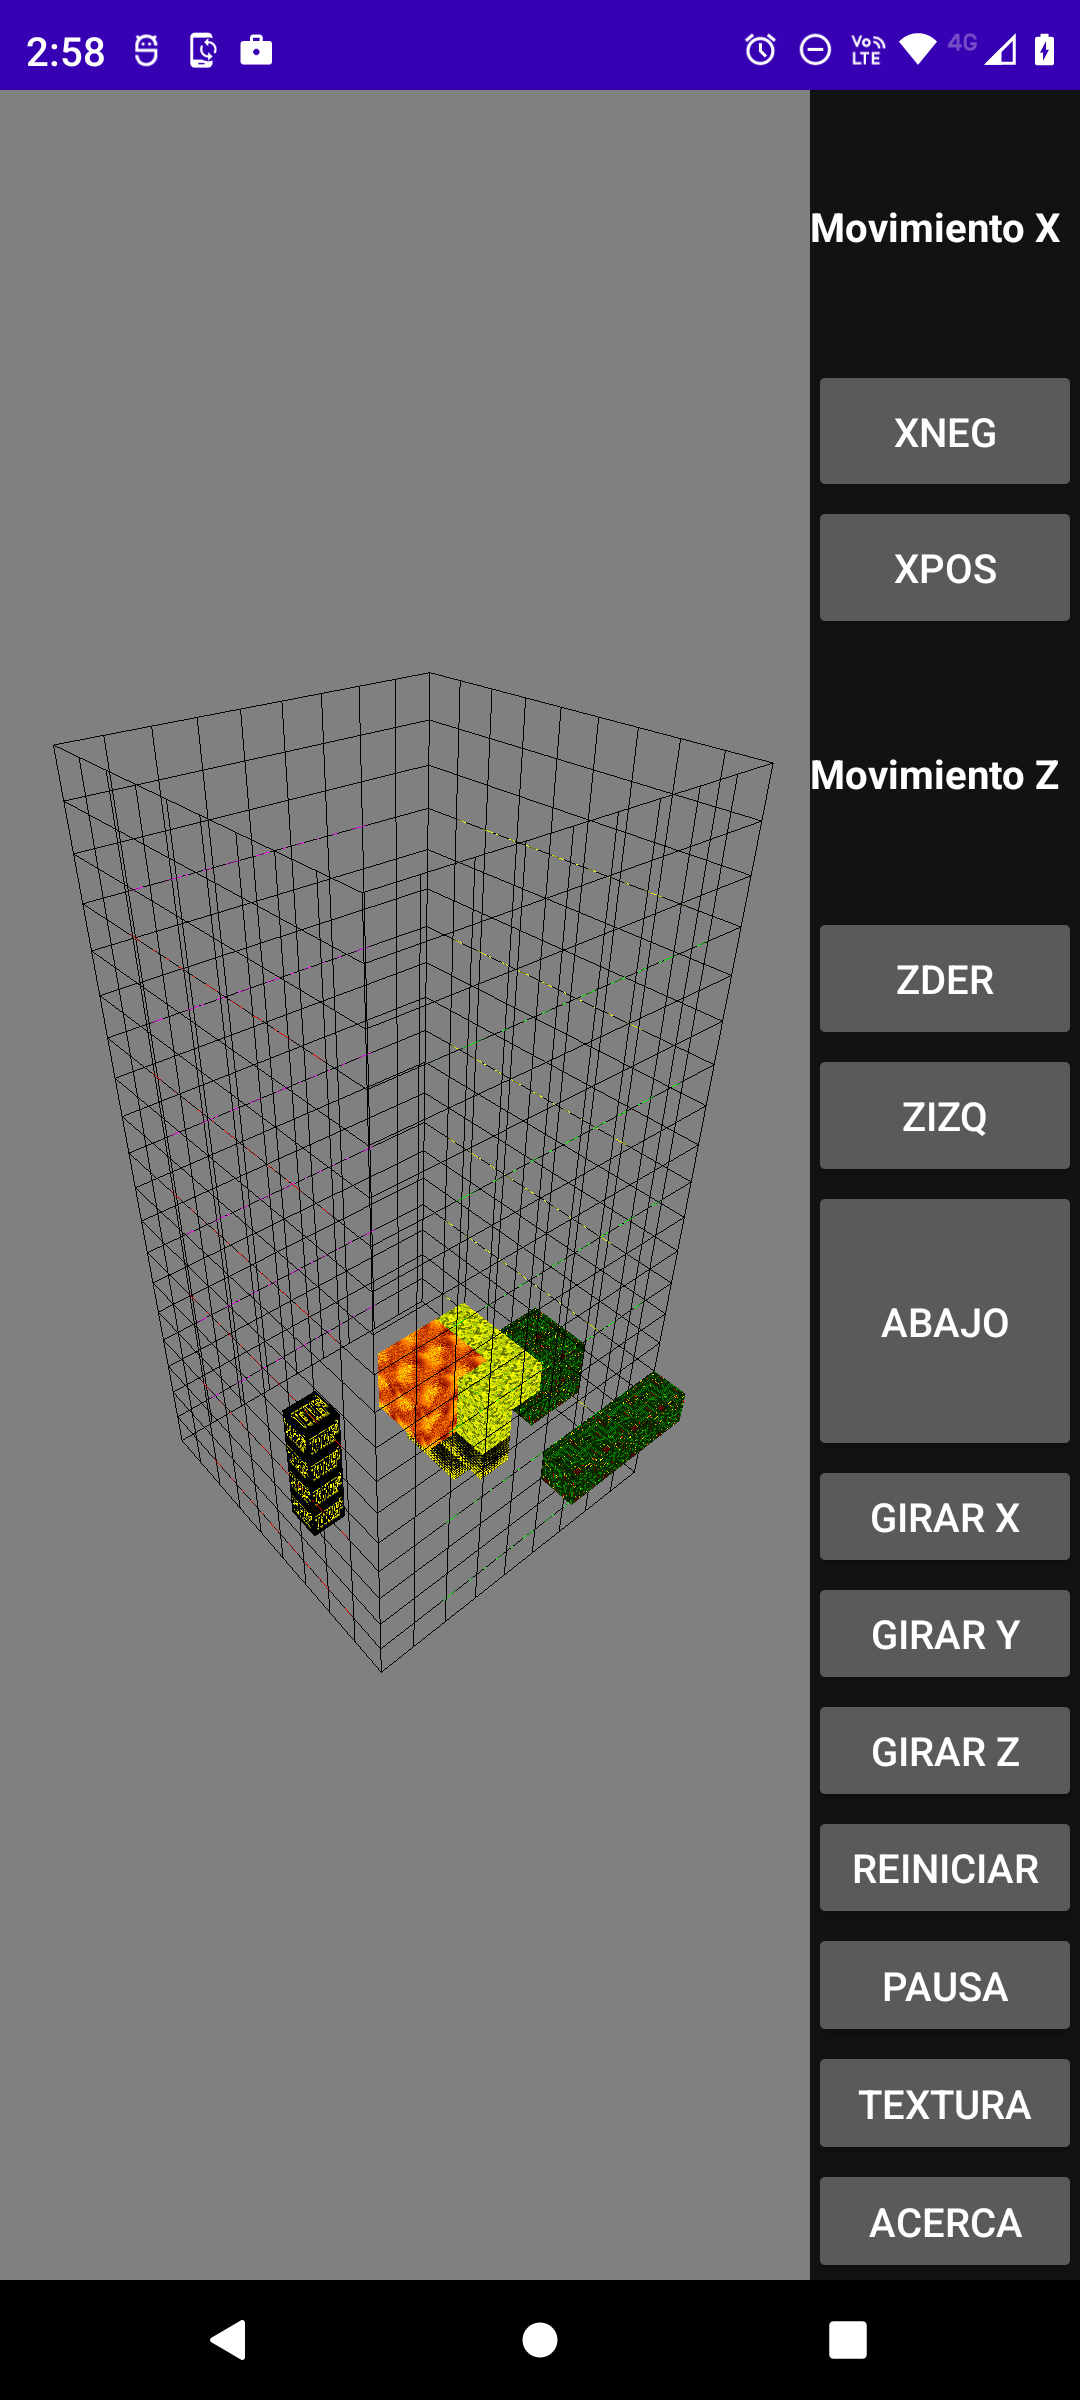
\includegraphics[width=0.20\linewidth]{2017_Tetris3D/figs/Tetris3.png} \\
	\end{tabular}
\end{center}
\end{frame}



